\documentclass[10pt, aspectratio=169]{beamer}

% -----------------------------------------------------------------------------
% Configuración del Tema y Estética Profesional
% -----------------------------------------------------------------------------
\usetheme{Madrid}
\usecolortheme{whale}

% Colores Personalizados (Estética Moderna y Elegante)
\definecolor{primaryblue}{RGB}{15, 34, 64}     % Azul marino profundo
\definecolor{secondaryblue}{RGB}{30, 80, 140}  % Azul intermedio
\definecolor{accentteal}{RGB}{0, 150, 136}    % Teal vibrante
\definecolor{darkgray}{RGB}{50, 50, 50}       % Gris oscuro para texto

\setbeamercolor{palette primary}{bg=primaryblue, fg=white}
\setbeamercolor{palette secondary}{bg=secondaryblue, fg=white}
\setbeamercolor{palette tertiary}{bg=primaryblue, fg=white}
\setbeamercolor{titlelike}{bg=primaryblue, fg=white}
\setbeamercolor{structure}{fg=primaryblue}
\setbeamercolor{block title}{bg=primaryblue, fg=white}
\setbeamercolor{block body}{bg=blue!5, fg=darkgray}
\setbeamercolor{block title alerted}{bg=red!80!black, fg=white}
\setbeamercolor{block body alerted}{bg=red!5, fg=darkgray}

% Desactivar barra de navegación inferior molesta
\setbeamertemplate{navigation symbols}{}
\setbeamertemplate{footline}[frame number]

% Paquetes esenciales
\usepackage[spanish]{babel}
\usepackage[utf8]{inputenc}
\usepackage{graphicx}
\usepackage{booktabs}
\usepackage{tikz}
\usepackage{tabularx}
\usepackage{multicol}
\usetikzlibrary{shapes, arrows, positioning, fit, backgrounds}

% Ruta de imágenes
\graphicspath{{figuras/}}

% -----------------------------------------------------------------------------
% INFORMACIÓN DE LA PORTADA
% -----------------------------------------------------------------------------
\title[Detección de Ataques Minoritarios IoT]{DETECCIÓN DE ATAQUES MINORITARIOS EN REDES IoT MEDIANTE UN MODELO HÍBRIDO BASADO EN STACKING, XGBOOST Y LIGHTGBM, PUNO 2026}
\subtitle{Sustentación de Tesis para Optar el Título Profesional de Ingeniera de Sistemas}
\author[Carmen Nieves Apaza Condori]{Bach. Carmen Nieves Apaza Condori}
\institute[UNAP]{
  Escuela Profesional de Ingeniería de Sistemas \\
  Facultad de Ingeniería Mecánica Eléctrica, Electrónica y Sistemas \\
  \textbf{Universidad Nacional del Altiplano - Puno}
}
\date{30 de Julio de 2026}

% -----------------------------------------------------------------------------
% DOCUMENTO PRINCIPAL DE DIAPOSITIVAS
% -----------------------------------------------------------------------------
\begin{document}

% -----------------------------------------------------------------------------
% SLIDE 1: PORTADA
% -----------------------------------------------------------------------------
\begin{frame}
  \titlepage
\end{frame}

% -----------------------------------------------------------------------------
% SLIDE 2: EL PROBLEMA CRÍTICO Y MOTIVACIÓN
% -----------------------------------------------------------------------------
\begin{frame}{El Problema Crítico: Sesgo Algorítmico y Desbalance en IoT}
\begin{columns}
  \begin{column}{0.52\textwidth}
    \begin{block}{Desbalance Extremo en Tráfico IoT ($\mathrm{IR} = 41.75:1$)}
      \small
      \begin{itemize}
        \item El \textbf{95.53\%} del tráfico corresponde a ataques volumétricos masivos (DDoS/DoS) y botnets.
        \item Los \textbf{ataques minoritarios infrecuentes} (\textit{Web-based} 0.14\% y \textit{Brute Force} 0.15\%) son los más destructivos pero quedan invisibilizados.
      \end{itemize}
    \end{block}
    
    \begin{alertblock}{La Paradoja de la Exactitud (Accuracy Paradox)}
      \small
      Los clasificadores tradicionales obtienen $>84\%$ de exactitud global simplemente por predecir la clase mayoritaria, pero sufren una \textbf{sensibilidad nula ($\mathrm{Recall} \to 0$)} en intrusiones críticas.
    \end{alertblock}
  \end{column}
  
  \begin{column}{0.45\textwidth}
    \centering
    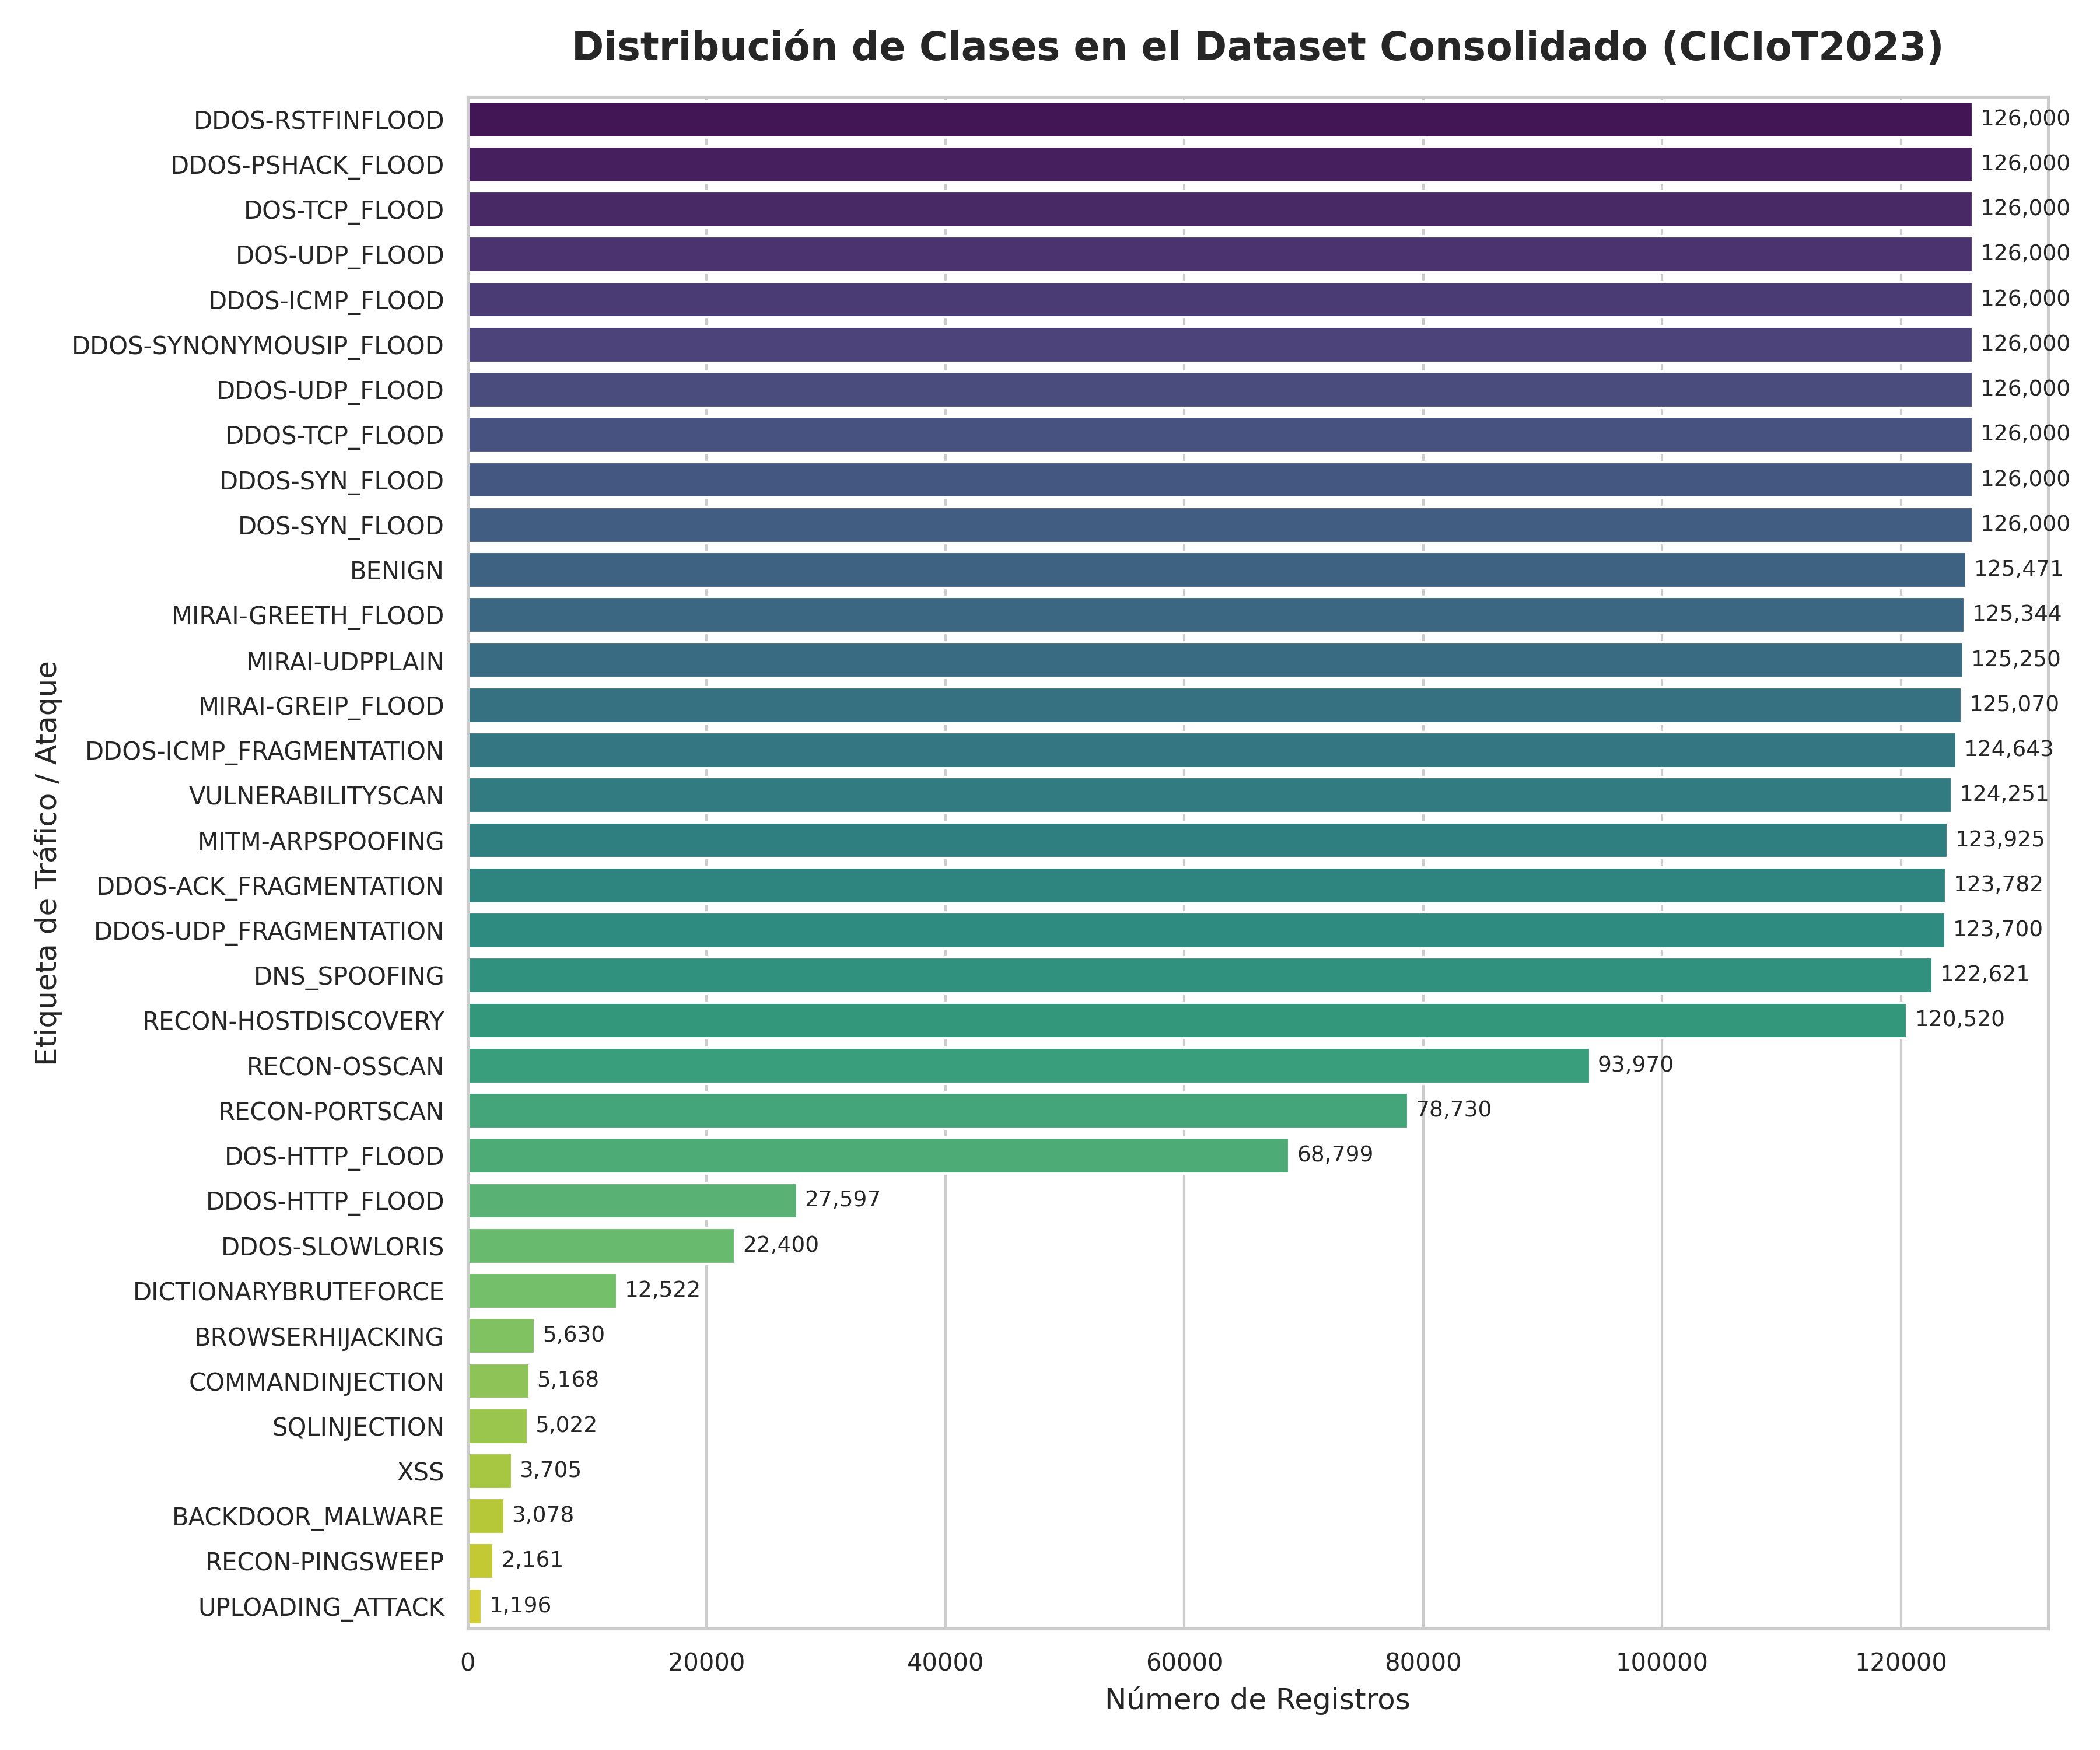
\includegraphics[width=\textwidth]{01_distribucion_clases.png} \\
    {\scriptsize Figura 1: Distribución asimétrica de clases en el dataset CICIoT2023.}
  \end{column}
\end{columns}
\end{frame}

% -----------------------------------------------------------------------------
% SLIDE 3: ARQUITECTURA PROPUESTA: STACKING HÍBRIDO CON ENTROPÍA
% -----------------------------------------------------------------------------
\begin{frame}{Solución Propuesta: Arquitectura Stacking Híbrida de 2 Niveles}
\vfill
\begin{center}
\resizebox{!}{0.75\textheight}{
\begin{tikzpicture}[
    node distance=0.5cm and 0.6cm,
    base/.style={rectangle, draw=primaryblue, thick, rounded corners=3pt, align=center, minimum height=0.7cm, font=\small, fill=blue!8},
    layer/.style={rectangle, draw=gray, dashed, inner sep=0.25cm},
    arrow/.style={->, >=stealth, thick, draw=primaryblue}
]

% Entrada
\node[base, fill=green!15, minimum width=9cm] (input) {\textbf{Entrada: Vector de 29 Características IoT} \\ {\scriptsize (Normalizado con \texttt{RobustScaler} y Rebalanceado con \texttt{Borderline-SMOTE1})}};

% Nivel 0
\node[base, fill=blue!15, below left=0.7cm and -1.8cm of input] (rf) {\textbf{Random Forest} \\ $P_{\mathrm{RF}}, H_{\mathrm{RF}}$};
\node[base, fill=blue!15, right=0.4cm of rf] (xgb) {\textbf{XGBoost GPU} \\ $P_{\mathrm{XGB}}, H_{\mathrm{XGB}}$};
\node[base, fill=blue!15, right=0.4cm of xgb] (lgb) {\textbf{LightGBM Base} \\ $P_{\mathrm{LGB}}, H_{\mathrm{LGB}}$};

\begin{pgfonlayer}{background}
\node[layer, fit=(rf) (xgb) (lgb), fill=gray!10, label={[anchor=south, font=\scriptsize]above:\textbf{Clasificadores de Nivel 0 (OOF 3-Fold)}}] (layer0) {};
\end{pgfonlayer}

% Extraccion de meta-features
\node[base, fill=yellow!20, minimum width=9cm, below=0.7cm of layer0] (meta) {\textbf{Tensor de Meta-Características $Z \in \mathbb{R}^{27}$} \\ {\scriptsize (24 Probabilidades + 3 Entropías de Shannon $H_{\mathrm{RF}}, H_{\mathrm{XGB}}, H_{\mathrm{LGB}}$)}};

% Nivel 1
\node[base, fill=red!15, minimum width=6cm, below=0.7cm of meta] (metalgb) {\textbf{Meta-Modelo (Nivel 1)} \\ LightGBM (\texttt{GridSearchCV})};

% Salida
\node[base, fill=green!15, minimum width=6cm, below=0.6cm of metalgb] (output) {\textbf{Predicción Final Multiclase} \\ {\scriptsize (8 Categorías de Tráfico IoT)}};

% Flechas
\draw[arrow] (input) -- (layer0);
\draw[arrow] (rf) -- (meta);
\draw[arrow] (xgb) -- (meta);
\draw[arrow] (lgb) -- (meta);
\draw[arrow] (meta) -- (metalgb);
\draw[arrow] (metalgb) -- (output);

\end{tikzpicture}
}
\end{center}
\vfill
\end{frame}

% -----------------------------------------------------------------------------
% SLIDE 4: PREPROCESAMIENTO Y SELECCIÓN DE ATRIBUTOS
% -----------------------------------------------------------------------------
\begin{frame}{Preprocesamiento y Selección de Atributos ($d=29$)}
\begin{columns}
  \begin{column}{0.48\textwidth}
    \centering
    \textbf{Higiene de Datos y Limpieza} \\
    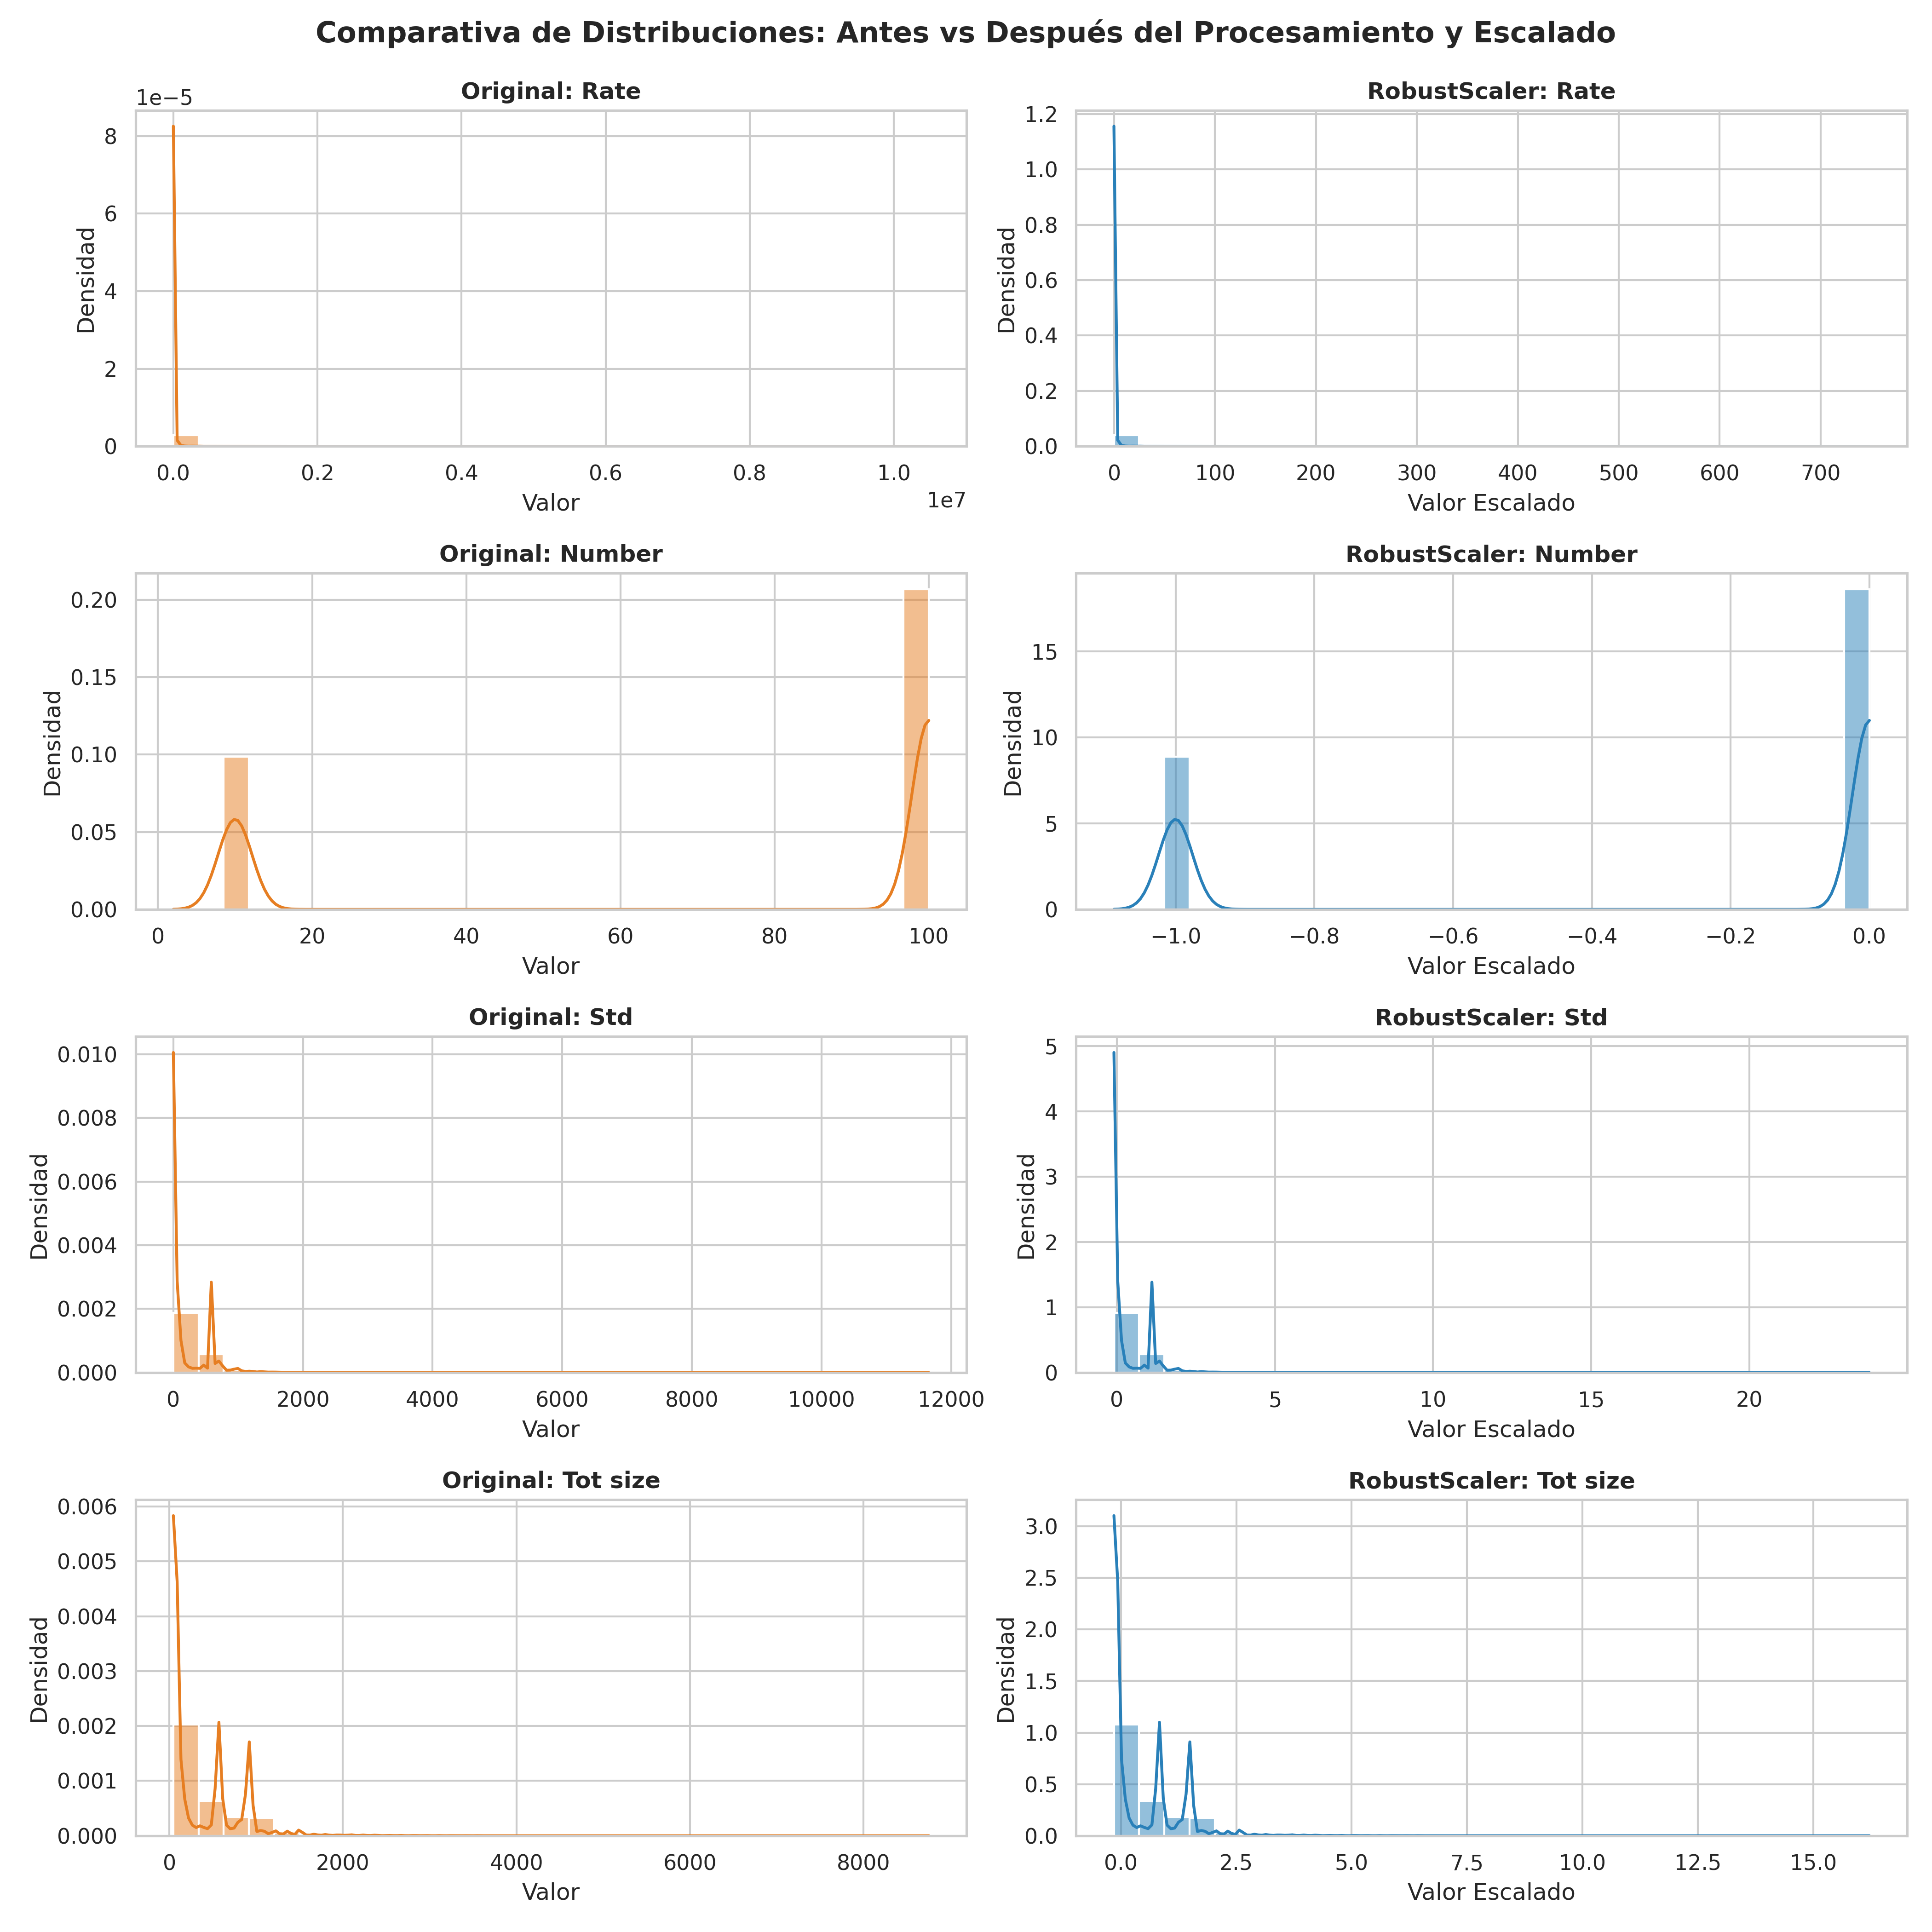
\includegraphics[width=0.95\textwidth]{05_comparacion_limpieza.png}
    \small
    \begin{itemize}
      \item Consolidación de 63 archivos CSV ($2.51$M flujos).
      \item Supresión de nulos (\texttt{NaN}), infinitos (\texttt{Inf}) y duplicados.
    \end{itemize}
  \end{column}
  
  \begin{column}{0.48\textwidth}
    \centering
    \textbf{Importancia por Impureza de Gini} \\
    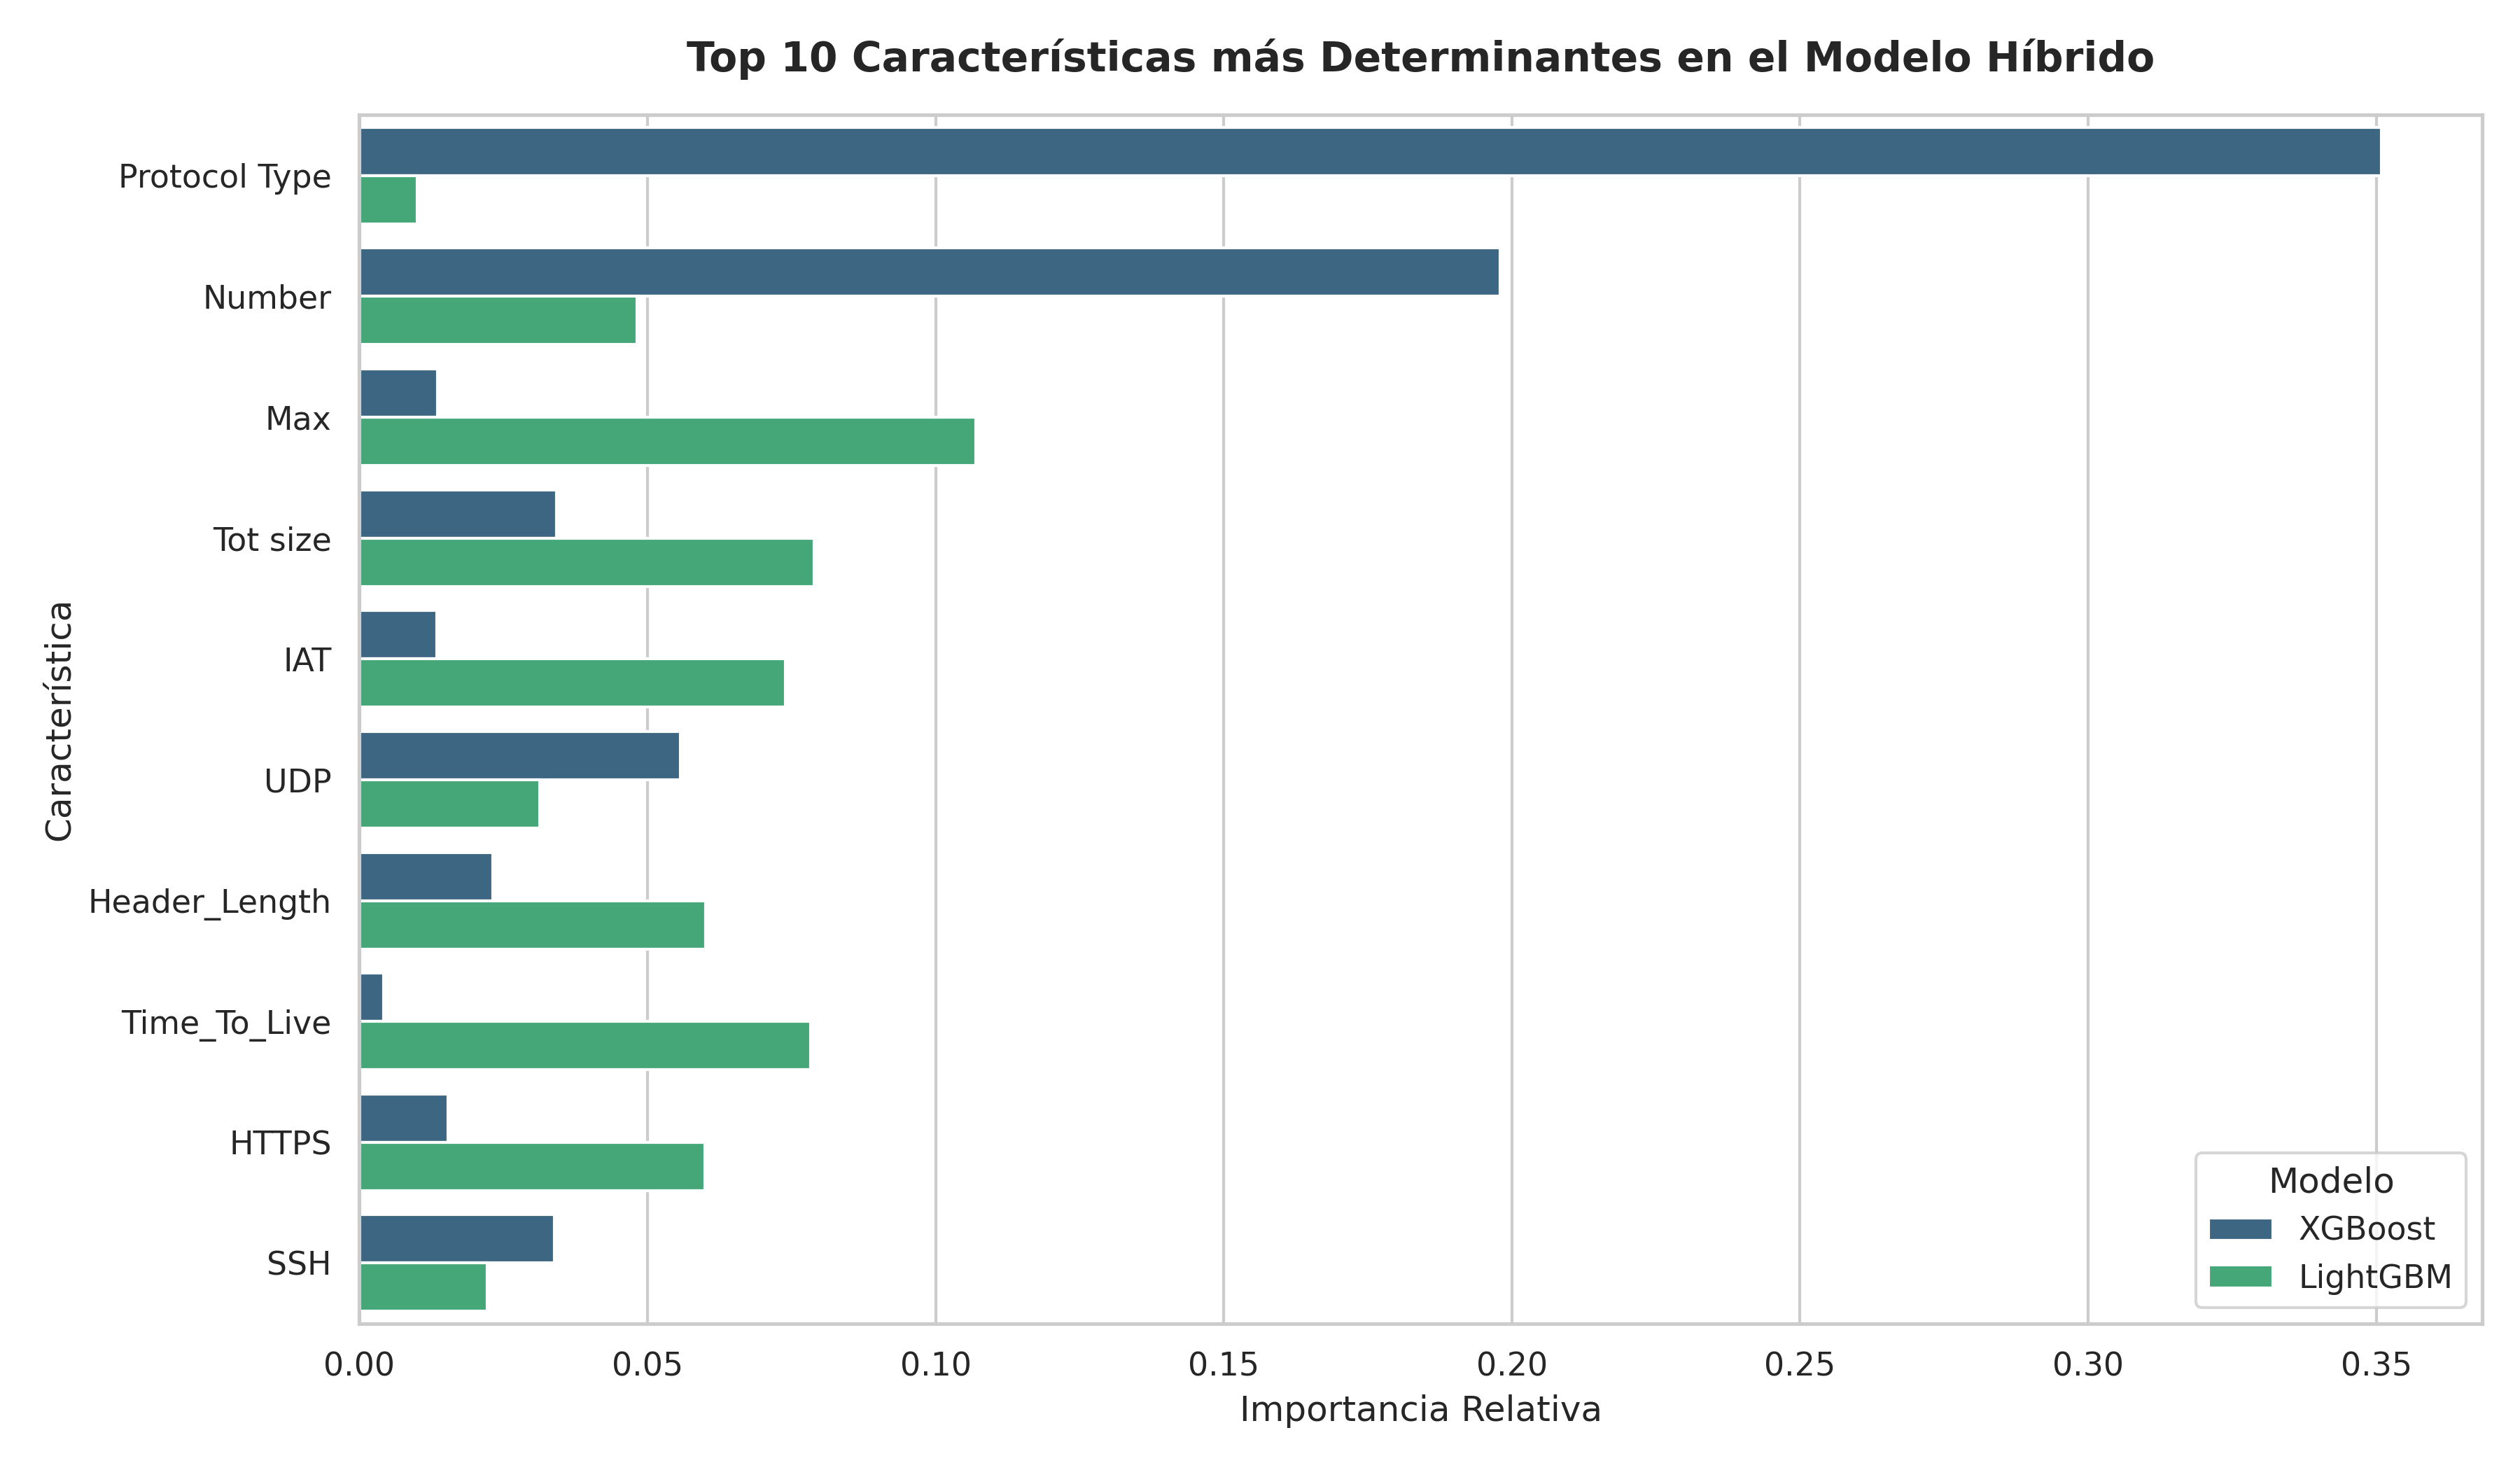
\includegraphics[width=0.95\textwidth]{12_importancia_caracteristicas.png}
    \small
    \begin{itemize}
      \item Selección de 29 variables continuas de red.
      \item Escalado Robusto con \texttt{RobustScaler} ($\mathrm{IQR}$).
    \end{itemize}
  \end{column}
\end{columns}
\end{frame}

% -----------------------------------------------------------------------------
% SLIDE 5: REBALANCEO SINTÉTICO EN LA FRONTERA (BORDERLINE-SMOTE1)
% -----------------------------------------------------------------------------
\begin{frame}{Sobremuestreo Adaptativo en la Frontera (Borderline-SMOTE1)}
\begin{columns}
  \begin{column}{0.55\textwidth}
    \centering
    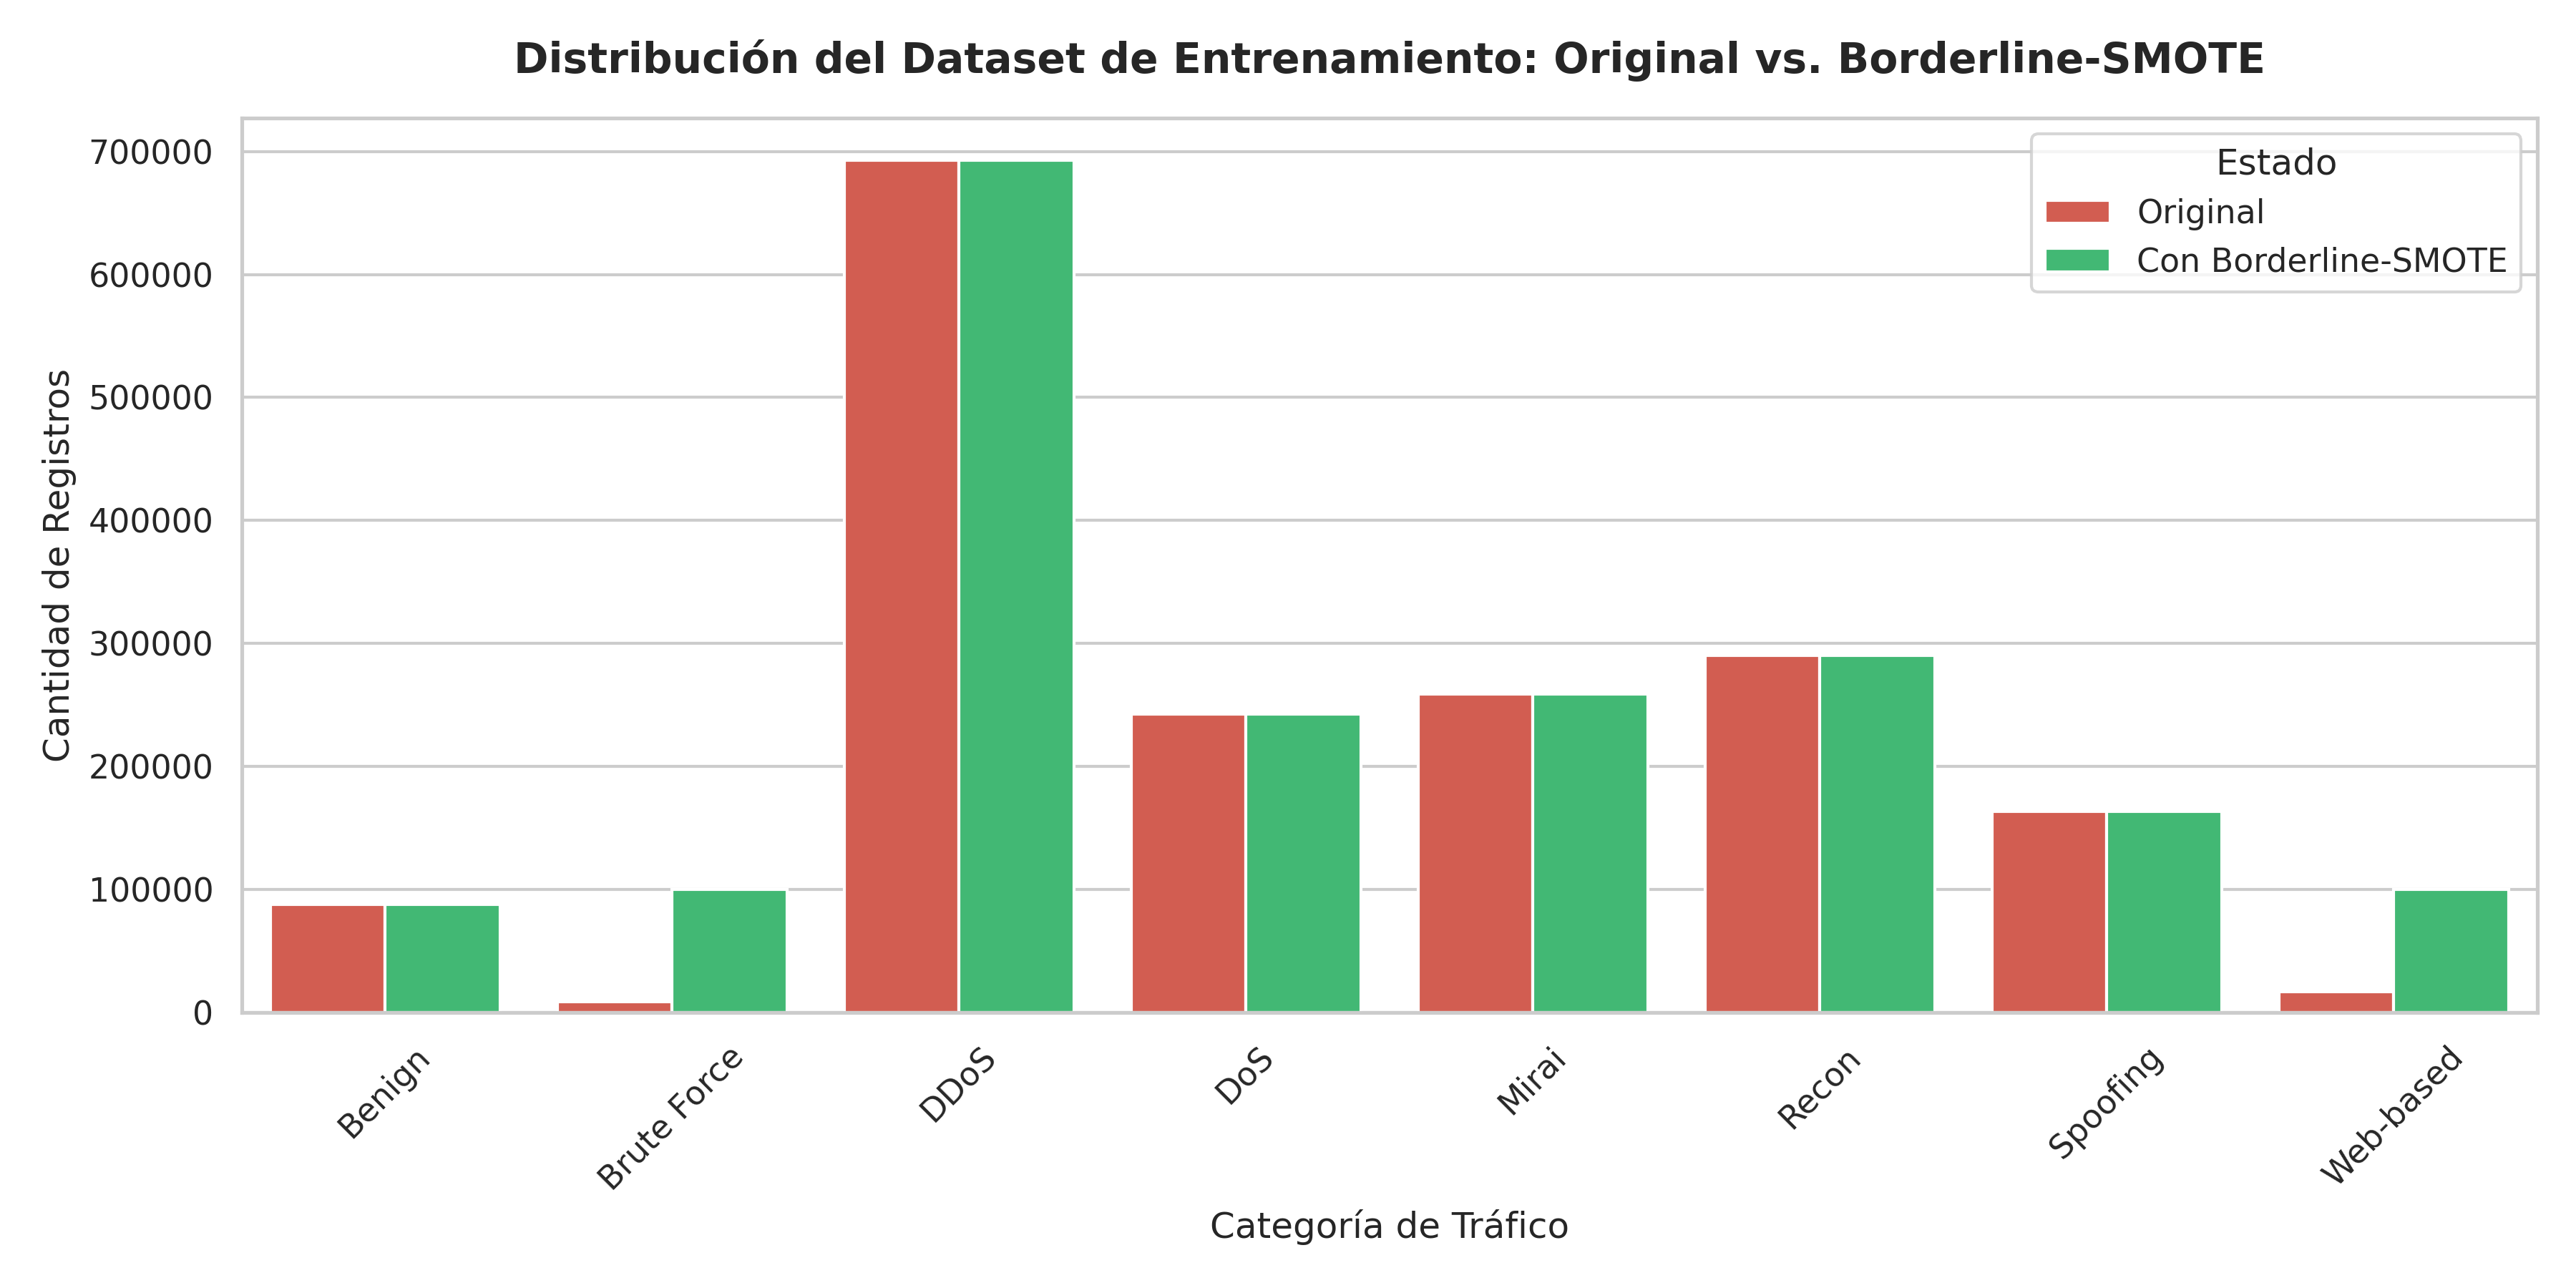
\includegraphics[width=\textwidth]{15_distribucion_borderline_smote.png}
  \end{column}
  
  \begin{column}{0.42\textwidth}
    \begin{block}{Generación Sintética Focalizada en $S_{\mathrm{danger}}$}
      \small
      \begin{itemize}
        \item Identifica muestras minoritarias en la frontera de decisión.
        \item Incrementa la presencia de \textit{Web-based} de \textbf{683 a 50,000 muestras} en entrenamiento.
        \item Evita la introducción de ruido sintético en regiones seguras.
      \end{itemize}
    \end{block}
  \end{column}
\end{columns}
\end{frame}

% -----------------------------------------------------------------------------
% SLIDE 6: RESULTADOS DE EFICACIA PREDICTIVA (EL NÚCLEO)
% -----------------------------------------------------------------------------
\begin{frame}{Resultados de Eficacia Predictiva sobre Test Set Aislado ($N=377,383$)}
\begin{columns}
  \begin{column}{0.52\textwidth}
    \small
    \begin{table}[H]
    \centering
    \resizebox{\textwidth}{!}{
    \begin{tabular}{l c c c}
      \toprule
      \textbf{Modelo Evaluado} & \textbf{F1-Macro} & \textbf{Accuracy} & \textbf{Recall} \\
      \midrule
      Regresión Logística & 0.4220 & 0.6120 & 0.4350 \\
      Árbol CART & 0.6651 & 0.8124 & 0.6590 \\
      Random Forest Base & 0.6791 & 0.8350 & 0.6750 \\
      LightGBM Base & 0.6953 & 0.8420 & 0.6910 \\
      XGBoost GPU Base & 0.6960 & 0.8435 & 0.6920 \\
      RF + Borderline-SMOTE & 0.6850 & 0.8290 & 0.6820 \\
      XGBoost + Borderline & 0.6995 & 0.8460 & 0.6950 \\
      \midrule
      \textbf{Stacking Híbrido} & \textbf{0.7018} & \textbf{0.8485} & \textbf{0.6980} \\
      \bottomrule
    \end{tabular}
    }
    \end{table}
    
    \begin{block}{Recuperación de Clases Minoritarias}
      \footnotesize
      \begin{itemize}
        \item \textit{Brute Force}: F1-Score elevado a \textbf{41.40\%}.
        \item \textit{Web-based}: F1-Score elevado a \textbf{33.86\%}.
      \end{itemize}
    \end{block}
  \end{column}
  
  \begin{column}{0.45\textwidth}
    \centering
    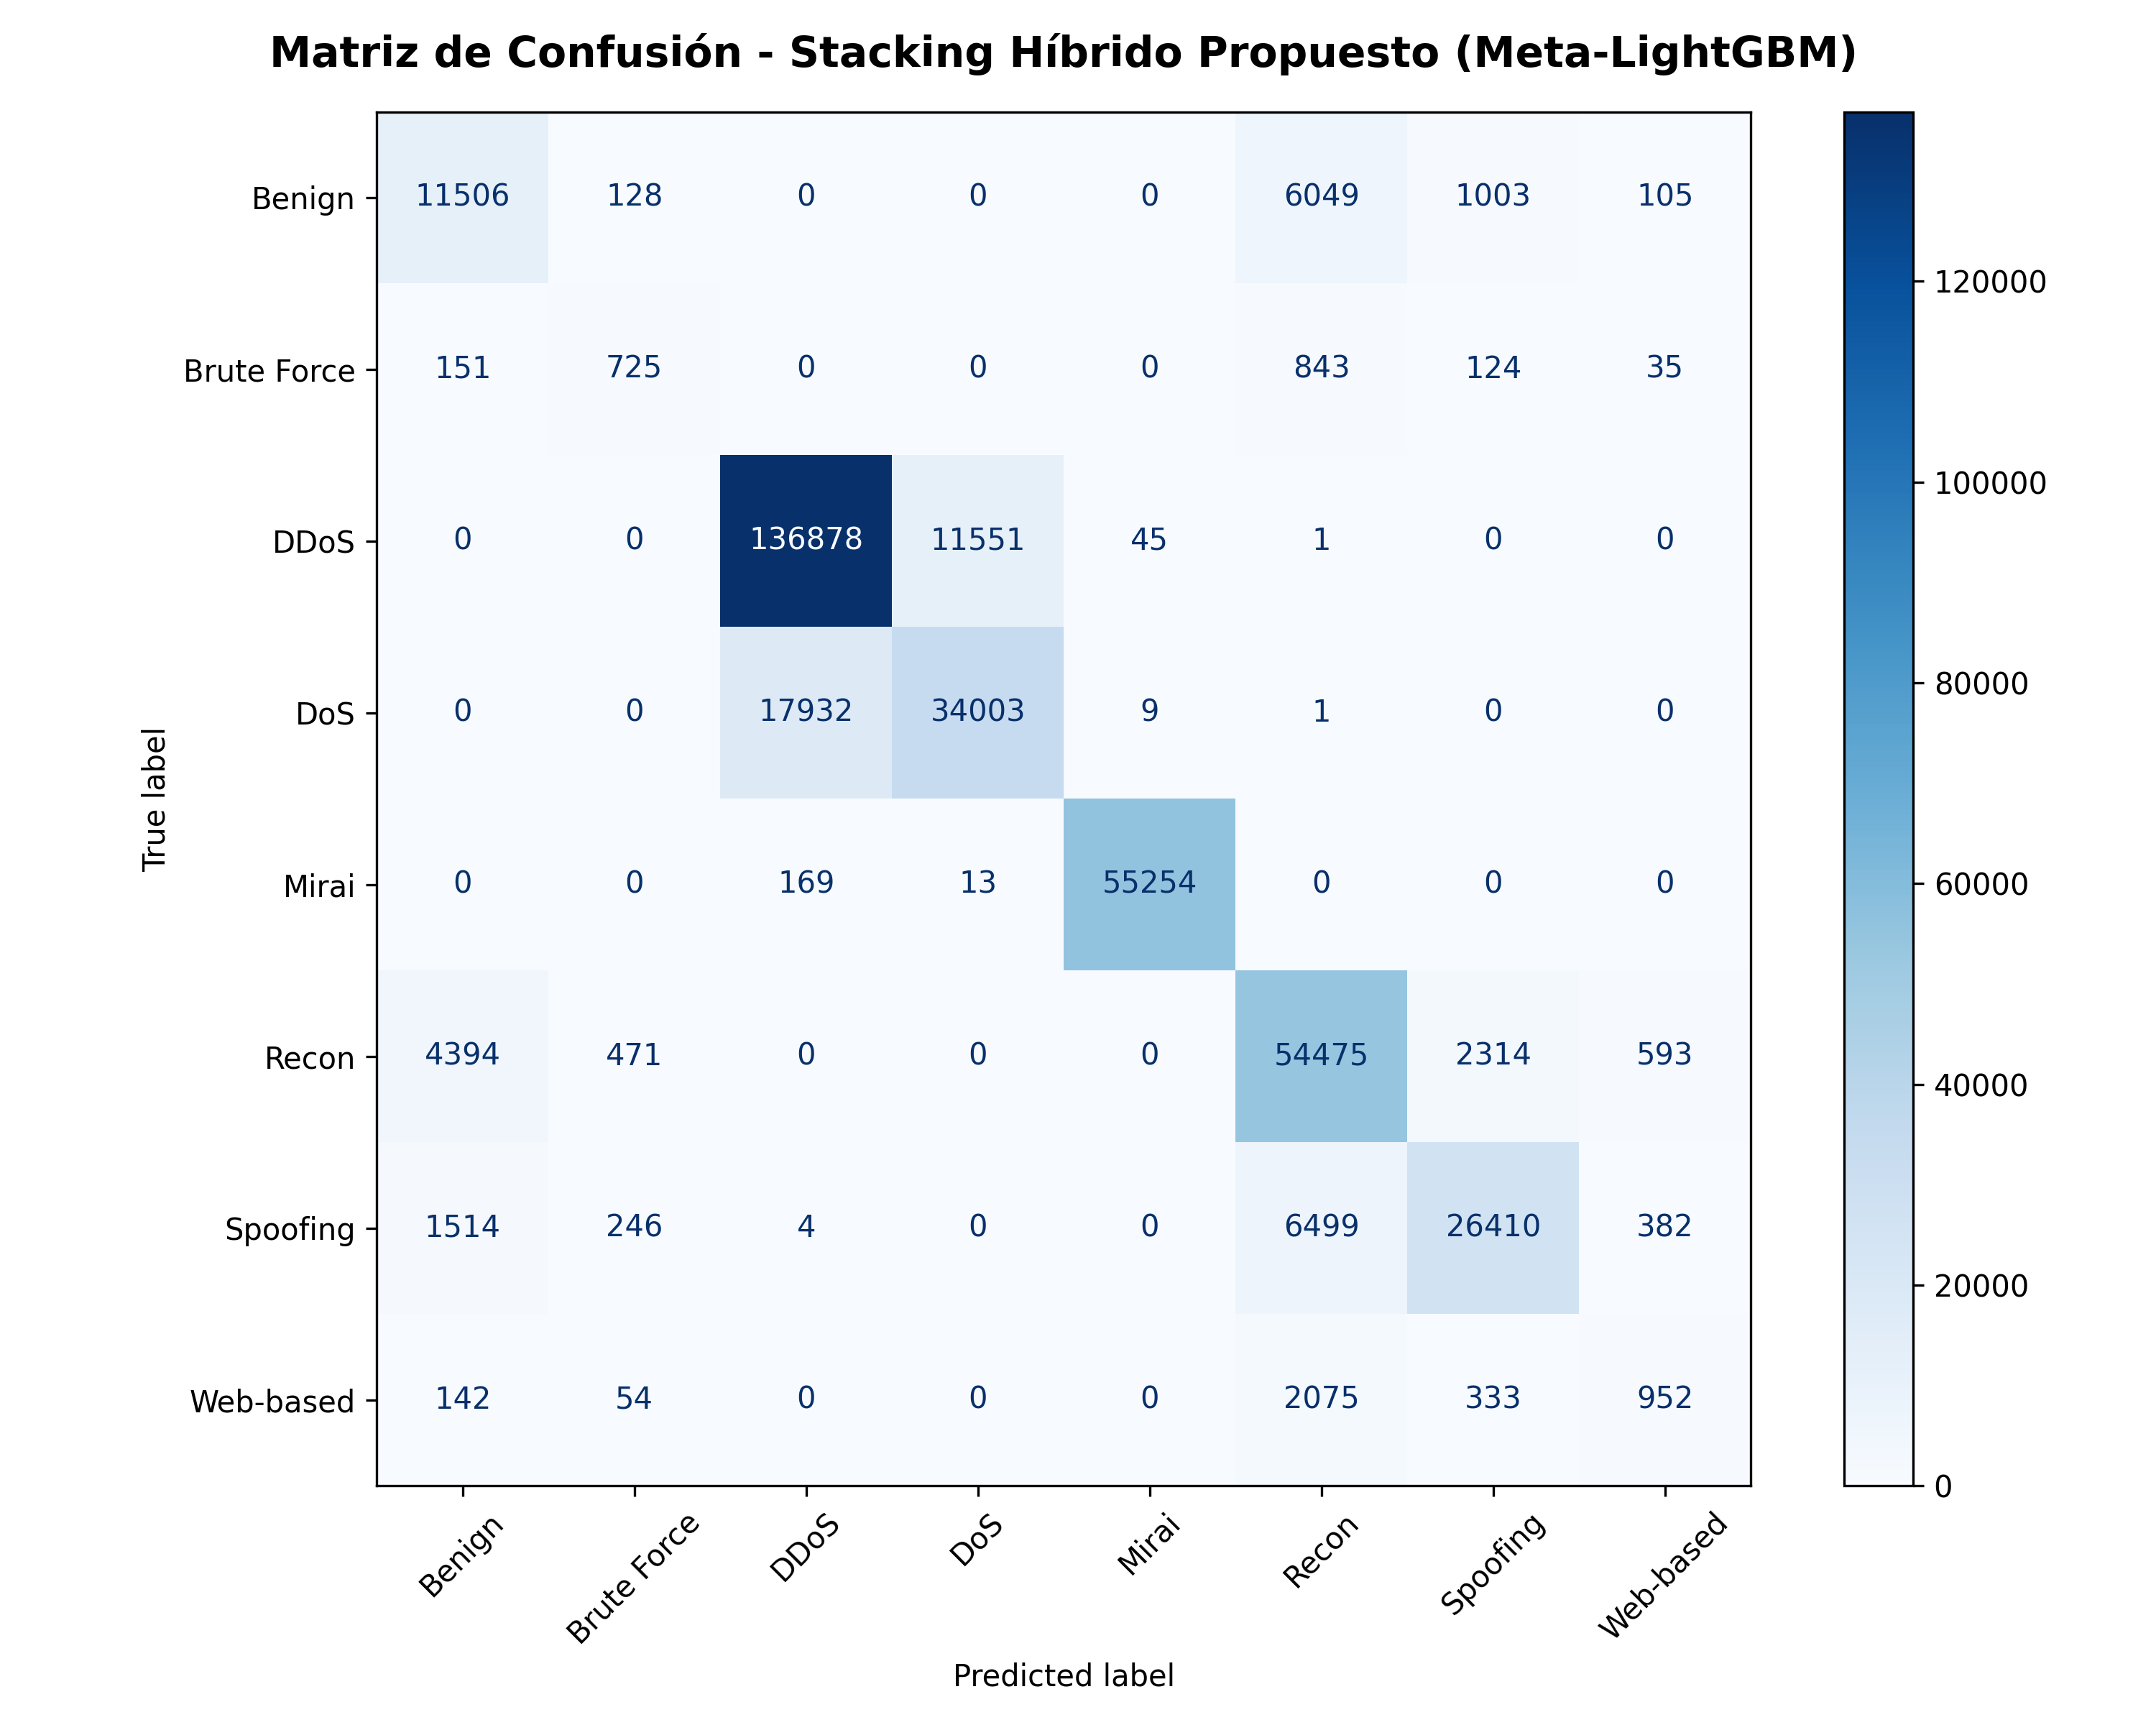
\includegraphics[width=\textwidth]{16_matriz_confusion_stacking_hibrido.png}
  \end{column}
\end{columns}
\end{frame}

% -----------------------------------------------------------------------------
% SLIDE 7: PERFILADO COMPUTACIONAL EN PASARELAS IOT
% -----------------------------------------------------------------------------
\begin{frame}{Perfilado Computacional de Viabilidad en Pasarelas IoT de Borde}
\begin{columns}
  \begin{column}{0.48\textwidth}
    \begin{block}{Métricas de Desempeño en Tiempo Real}
      \small
      \begin{itemize}
        \item \textbf{Latencia por Muestra:} $8.65\,\mu s$
        \item \textbf{Tasa de Procesamiento:} $115,613$ paquetes por segundo.
        \item \textbf{Ocupación de RAM:} $257.89\text{ MB}$ (Cumple $<300\text{ MB}$).
      \end{itemize}
    \end{block}
  \end{column}
  
  \begin{column}{0.48\textwidth}
    \begin{alertblock}{Ventaja frente a Deep Learning (CNN/LSTM)}
      \small
      \begin{itemize}
        \item Redes profundas exigen latencias $>100\,\mu s$ y GPUs de alto consumo.
        \item El Stacking es \textbf{liviano, eficiente e interoperable} para pasarelas de borde (Raspberry Pi / Jetson Nano) vía ONNX.
      \end{itemize}
    \end{alertblock}
  \end{column}
\end{columns}
\end{frame}

% -----------------------------------------------------------------------------
% SLIDE 8: PRUEBA ESTADÍSTICA DE WILCOXON
% -----------------------------------------------------------------------------
\begin{frame}{Validación Estadística de Significancia (Prueba de Wilcoxon)}
\begin{columns}
  \begin{column}{0.55\textwidth}
    \centering
    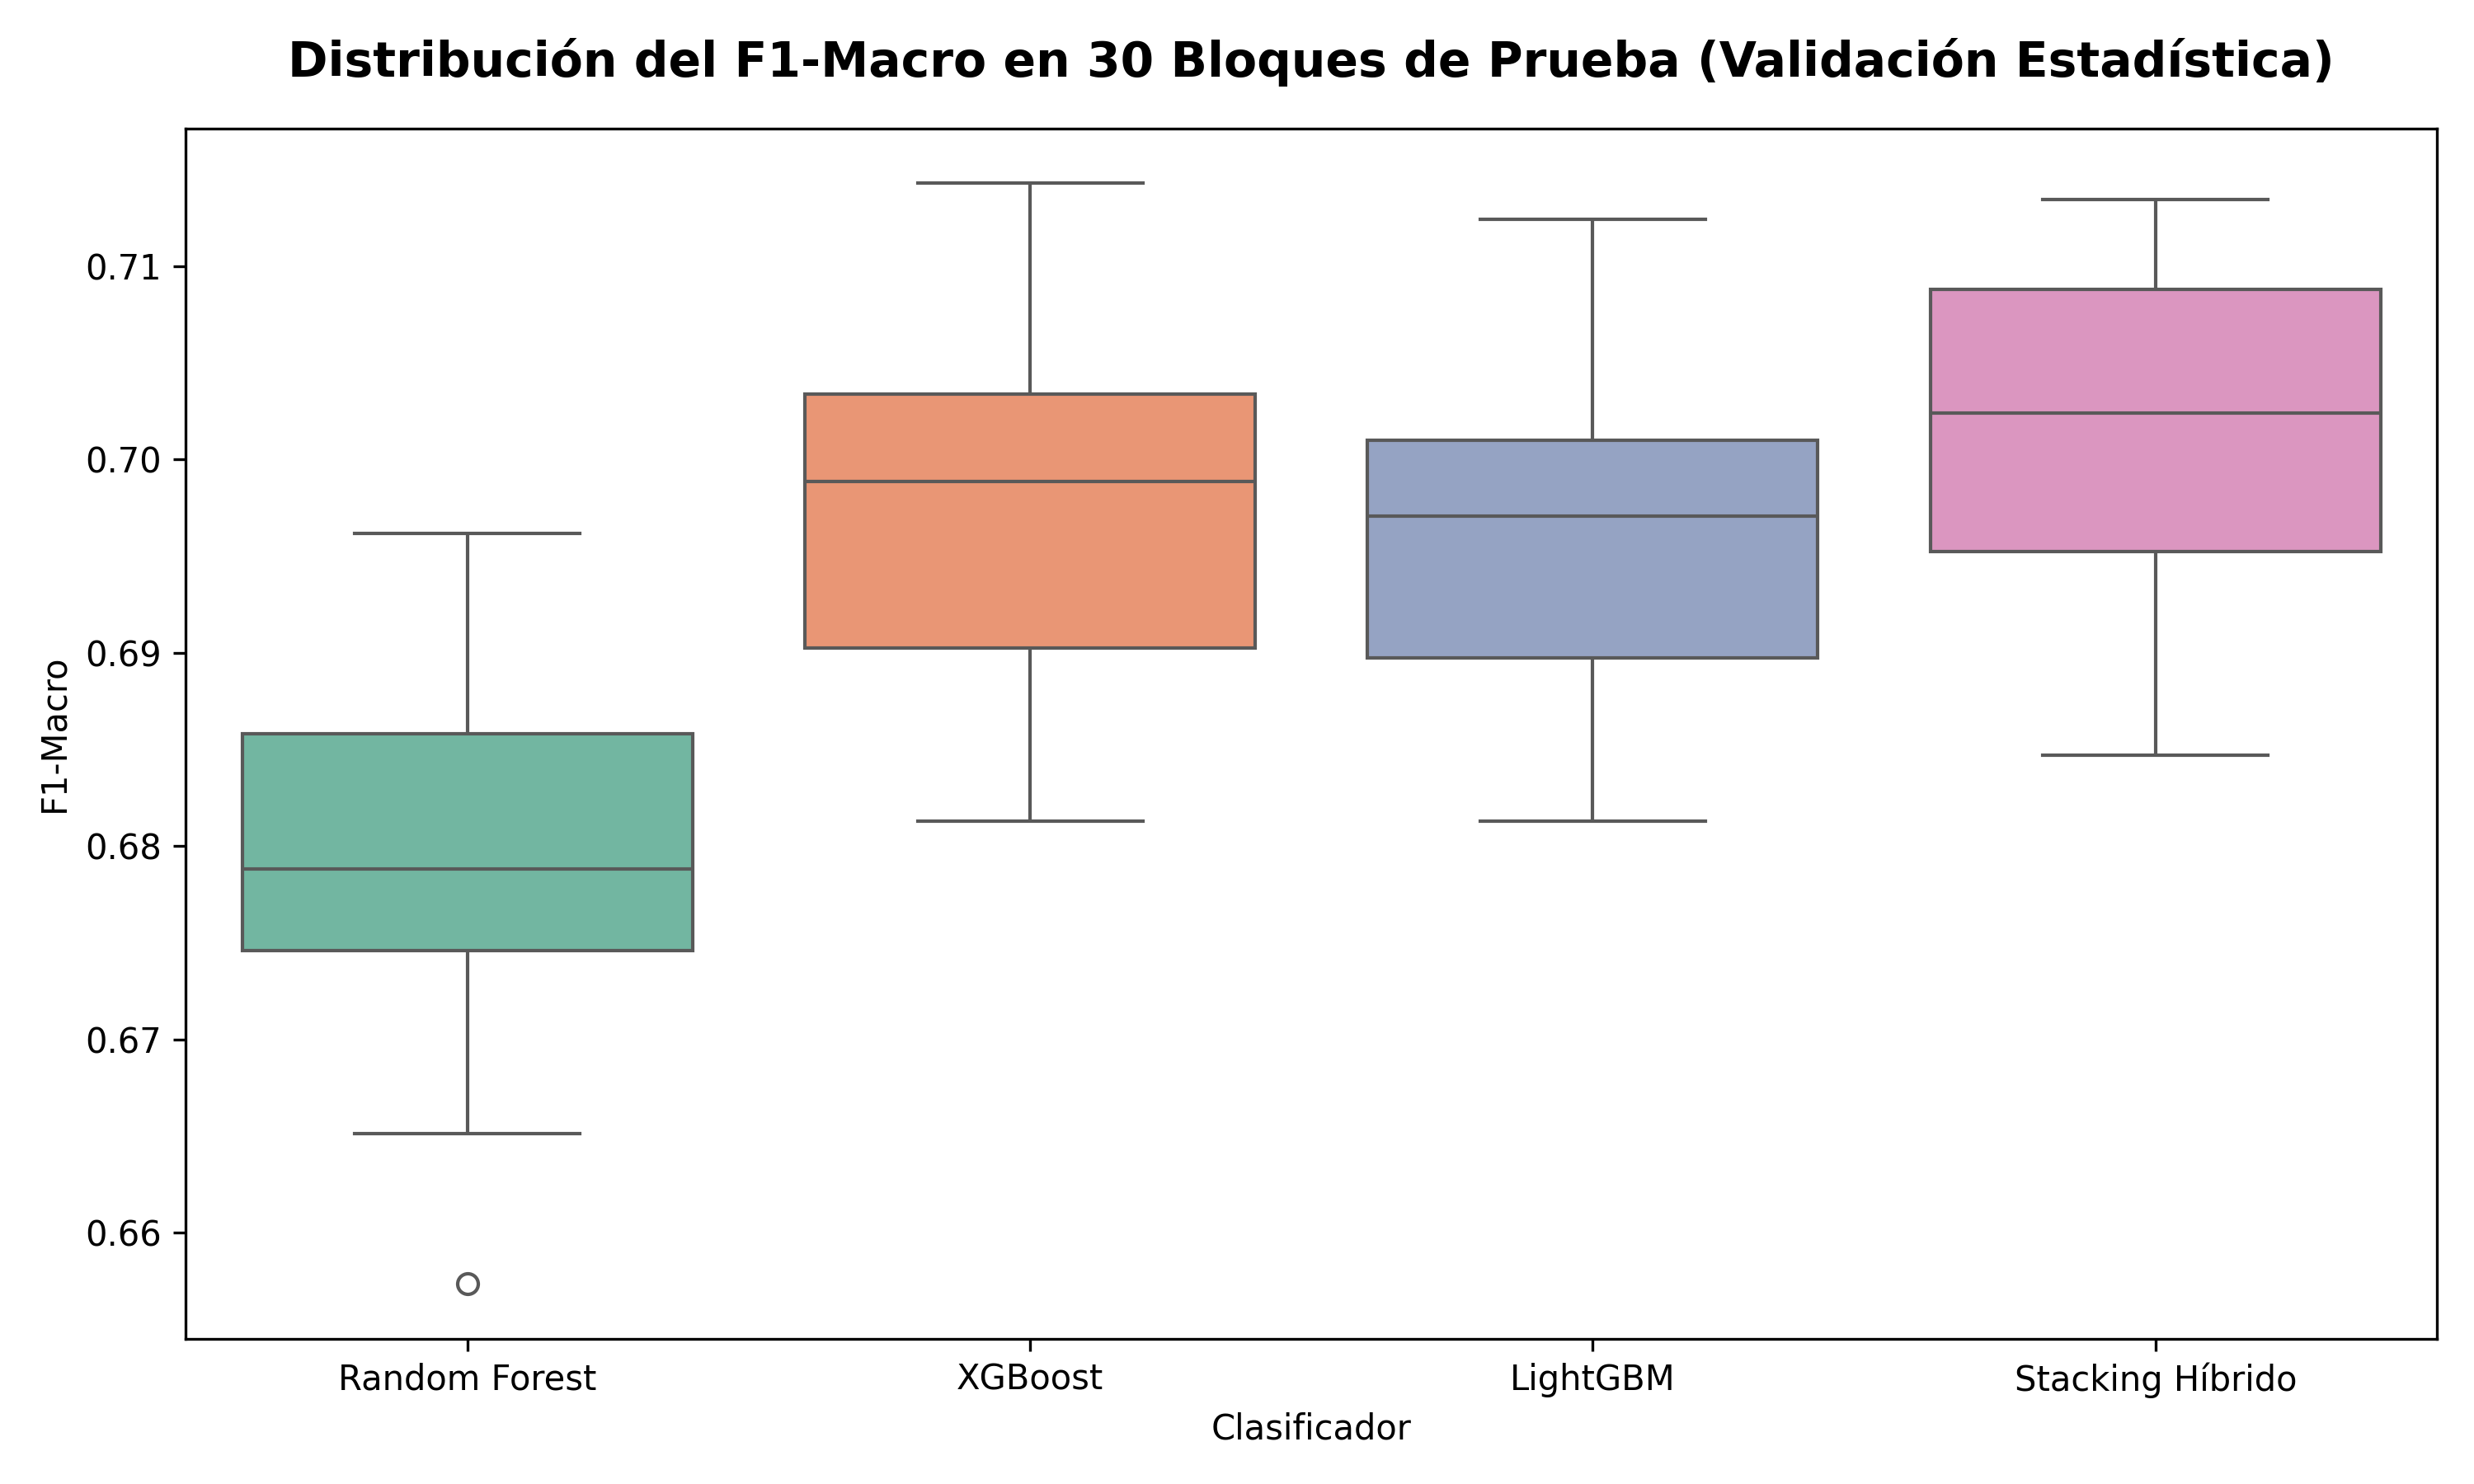
\includegraphics[width=\textwidth]{18_boxplot_wilcoxon.png}
  \end{column}
  
  \begin{column}{0.42\textwidth}
    \small
    \begin{block}{Prueba de Wilcoxon (30 Bloques)}
      \footnotesize
      \begin{itemize}
        \item $W^+ = 95.0$
        \item \textbf{$p$-valor $= 0.003744 < 0.05$}
      \end{itemize}
    \end{block}
    
    \begin{alertblock}{Conclusión Estadística}
      \footnotesize
      Se rechaza la Hipótesis Nula ($H_0$) y se acepta la \textbf{Hipótesis General ($H_G$)} con un nivel de confianza del \textbf{99.5\%}.
    \end{alertblock}
  \end{column}
\end{columns}
\end{frame}

% -----------------------------------------------------------------------------
% SLIDE 9: CONCLUSIONES Y CONTRIBUCIONES
% -----------------------------------------------------------------------------
\begin{frame}{Conclusiones Principales y Aportes}
\small
\begin{enumerate}
  \item \textbf{Eficacia y Generalización:} La arquitectura Stacking con Entropía de Shannon alcanza un F1-Macro del \textbf{70.18\%} y Accuracy del \textbf{84.85\%}, superando estadísticamente a todos los modelos de control.
  \item \textbf{Neutralización del Sesgo:} \texttt{Borderline-SMOTE1} y \texttt{RobustScaler} mitigan la paradoja de la exactitud, elevando la sensibilidad en intrusiones minoritarias (\textit{Brute Force} a 41.40\% y \textit{Web-based} a 33.86\%).
  \item \textbf{Viabilidad en Borde:} La latencia de \textbf{$8.65\,\mu s$} y consumo de \textbf{$257.89\text{ MB}$ RAM} garantizan su despliegue operativo en pasarelas IoT de MYPEs y PYMEs.
\end{enumerate}
\end{frame}

% -----------------------------------------------------------------------------
% SLIDE 10: AGRADECIMIENTO Y CIERRE
% -----------------------------------------------------------------------------
\begin{frame}{¡Muchas Gracias por su Atención!}
\begin{center}
  \Large \textbf{¿Preguntas o Comentarios del Jurado Evaluador?}
  
  \vspace{1cm}
  \normalsize
  \textbf{Repositorio Oficial del Proyecto en GitHub:} \\
  \small \url{https://github.com/carmenNieves6478/DETECCI-N-DE-ATAQUES-MINORITARIOS-EN-REDES-IoT-MEDIANTE-UN-MODELO-H-BRIDO.git}
  
  \vspace{0.8cm}
  \small \textbf{Bach. Carmen Nieves} \\
  Universidad Nacional del Altiplano - Puno
\end{center}
\end{frame}

\end{document}
